%%%%%%%%%%%%%%%%%%%%%%%%%%%%%%%%%%%%%%%%%%%%%%%%%%%%%%%%%%%%%%%%%%%%%%%%%%%%%%%%
%% Introductions
%%%%%%%%%%%%%%%%%%%%%%%%%%%%%%%%%%%%%%%%%%%%%%%%%%%%%%%%%%%%%%%%%%%%%%%%%%%%%%%%


\section{Introduction}

%%%%%%%%%%%%%%%%%%%%%%%%%%%%%%%%%%%%%%%%%%%%%%%%%%%%%%%%%%%%%%%%%%%%%%%%%%%%%%%%
%%%%    Background

\subsection{Background and clinical significance}

	Heart valve treatment is a common cardiovascular surgical procedure with over 100,800 done annually in the U.S. alone \cite{mozaffarian_heart_2016} and 275,000 to 370,000 in developed nations \cite{manji_future_2012}. Almost all contemporary heart valve replacement designs use exogenously crosslinked (EXL) collagenous soft tissues (e.g. bovine pericardium) to manufacture leaflets for bioprosthetic valves (BHVs) \cite{starr_artificial_2007, soares_biomechanical_2016}. BHVs have advantages in immunogenicity and hemodynamics over other designs, but also have a limited life span of 10-15 years. As a recent development in BHV technology, transcatheter valve interventions \cite{bonow_accaha_2006, guidoin_marvel_2010} reduce surgical risk and make valve replacement more feasible for those who cannot tolerate full surgical interventions. However, this new technology also presents additional design challenges, including complex folding and compression during delivery. As a result, the leaflets are required to be significantly thinner than in traditional BHVs, which increases the leaflet stress and potentially the rate of failure. Existing data on transcatheter aortic valve interventions suggest a 2-year mortality rate of 33.9\% overall \cite{mozaffarian_heart_2016} and over 68\% when specifically replacing stenotic aortic valves \cite{makkar_transcatheter_2012}. As such, this further accentuates the need to develop an approach to improve BHV durability. 
	
%%%%%%%%%%%%%%%%%%%%%%%%%%%%%%%%%%%%%%%%%%%%%%%%%%%%%%%%%%%%%%%%%%%%%%%%%%%%%%%%
%%%%    Failure
	 
\subsection{Mechanisms of BHV failure}

	The causes of BHV failure can be divided into two broad categories, mineralization and structural damage, with both processes occurring in parallel or independently \cite{sacks_collagen_2002}. Mineralization is the accumulation of mineral deposits, mainly calcium phosphate, within the BHV leaflets \cite{schoen_calcification_2005}. This disrupts the underlying microstructure preventing the proper mechanical function of BHVs, increasing the likelihood of tearing, and reducing flexibility (preventing normal opening and closing motions, and induce valve stenosis). This process is exacerbated by the presence of exogenous crosslinkers, such as glutaraldehyde (GLUT), where the phosphates from the devitalized endothelial cells bind with the calcium in blood to form deposits. The causes of calcification and associated anti-calcification treatments are extensively studied in literature \cite{park_novel_1997, isenburg_tannic_2005, vyavahare_prevention_1997}. On the other hand, structural damage includes the collagen fiber damage and breakdown of the non-fibrous part of extracellular matrix (ECM), \emph{which we will refer as simply the matrix}. Fourier transform infrared spectroscopy(FTIR) results have shown changes in the collagen fiber molecular structure after 50 million cycles \cite{sun_response_2004}, which suggests that some collagen fiber damage has occurred during this period. However, its effect on the mechanical response of BHVs was not detectable. Nevertheless, it is important to maintain the structural integrity of the BHV, as this will help to improve BHV durability. 
	
%%%%%%%%%%%%%%%%%%%%%%%%%%%%%%%%%%%%%%%%%%%%%%%%%%%%%%%%%%%%%%%%%%%%%%%%%%%%%%%%
%%%%    Cyclic loading
	
\subsection{Response to long-term cyclic loading}

	The current process for evaluating BHV designs is an expensive and time consuming three-stage process: 1) accelerated wear testing(AWT), 2) large animal studies, and 3) clinical trials. AWT is performed by cycling BHVs in sterile saline at 10 to 20 times the normal heart rate. It is currently the only way to evaluate BHV durability in a feasible amount of time (months instead of years). However, the loading conditions and environment during AWT are not physiological and the only durability information currently used is the presence of visible damage. Designs which show promise are then put through costly large animal studies, which still do not fully duplicate the human native environment. The final and most important stage is clinical evaluations. This is the only stage in evaluation process that can provide true indications of the \textit{in vivo} performance of BHV designs. However, this is the final, most difficult, most expensive and most time consuming stage. Clearly, current methods of evaluating BHV designs are not feasible for advancing the BHV technology in a timely manner. Computational simulations have been presented as an effective approach to this problem\cite{soares_biomechanical_2016}. To be effective, we need better a understanding of the underlying mechanisms of structural damage. 
	

	However, these mechanisms are poorly understood, especially for how they affect the mechanical response of the exogenously crosslinked tissues used to construct the BHV leaflets. The most significant change in response to cyclic loading is the change in geometry of the BHV leaflets. In a study on the porcine aortic BHVs \cite{smith_high_1997},  Smith \textit{et al}. found significant changes in the unloaded geometry of BHVs after AWT, especially in the belly region of the leaflets (Fig. \ref{fig:PSeffects}A). By changing the unloaded reference configuration, the shape of the leaflets and their mechanical response will change as well. Further analysis shown that significant structure damage occurred within the belly region as compared to other regions of the leaflet, where the stress significantly increased \cite{smith_fatigue_1999}. Interestingly, Smith et al. also found most the most significant changes in BHV leaflet geometry to occur within first 50 million cycles \cite{smith_high_1997}. Moreover, Sacks and Smith \cite{sacks_effects_1998} also found that there were minimal structural damage in this early stage (Fig. \ref{fig:PSeffects}B). This is further supported by another study by Wells \textit{et al} \cite{wells_cyclic_2005}, where they found minimal structural changes during the first 50 million cycles for the pressure fixed BHVs, with most significant change observed in the first million cycles. Clearly, there is a non-damage based mechanism at play that changes the geometry of the material, with significant impact on the early stage of cycling and the rate of fatigue in later stages. 


\begin{figure}[hbt]
\centering
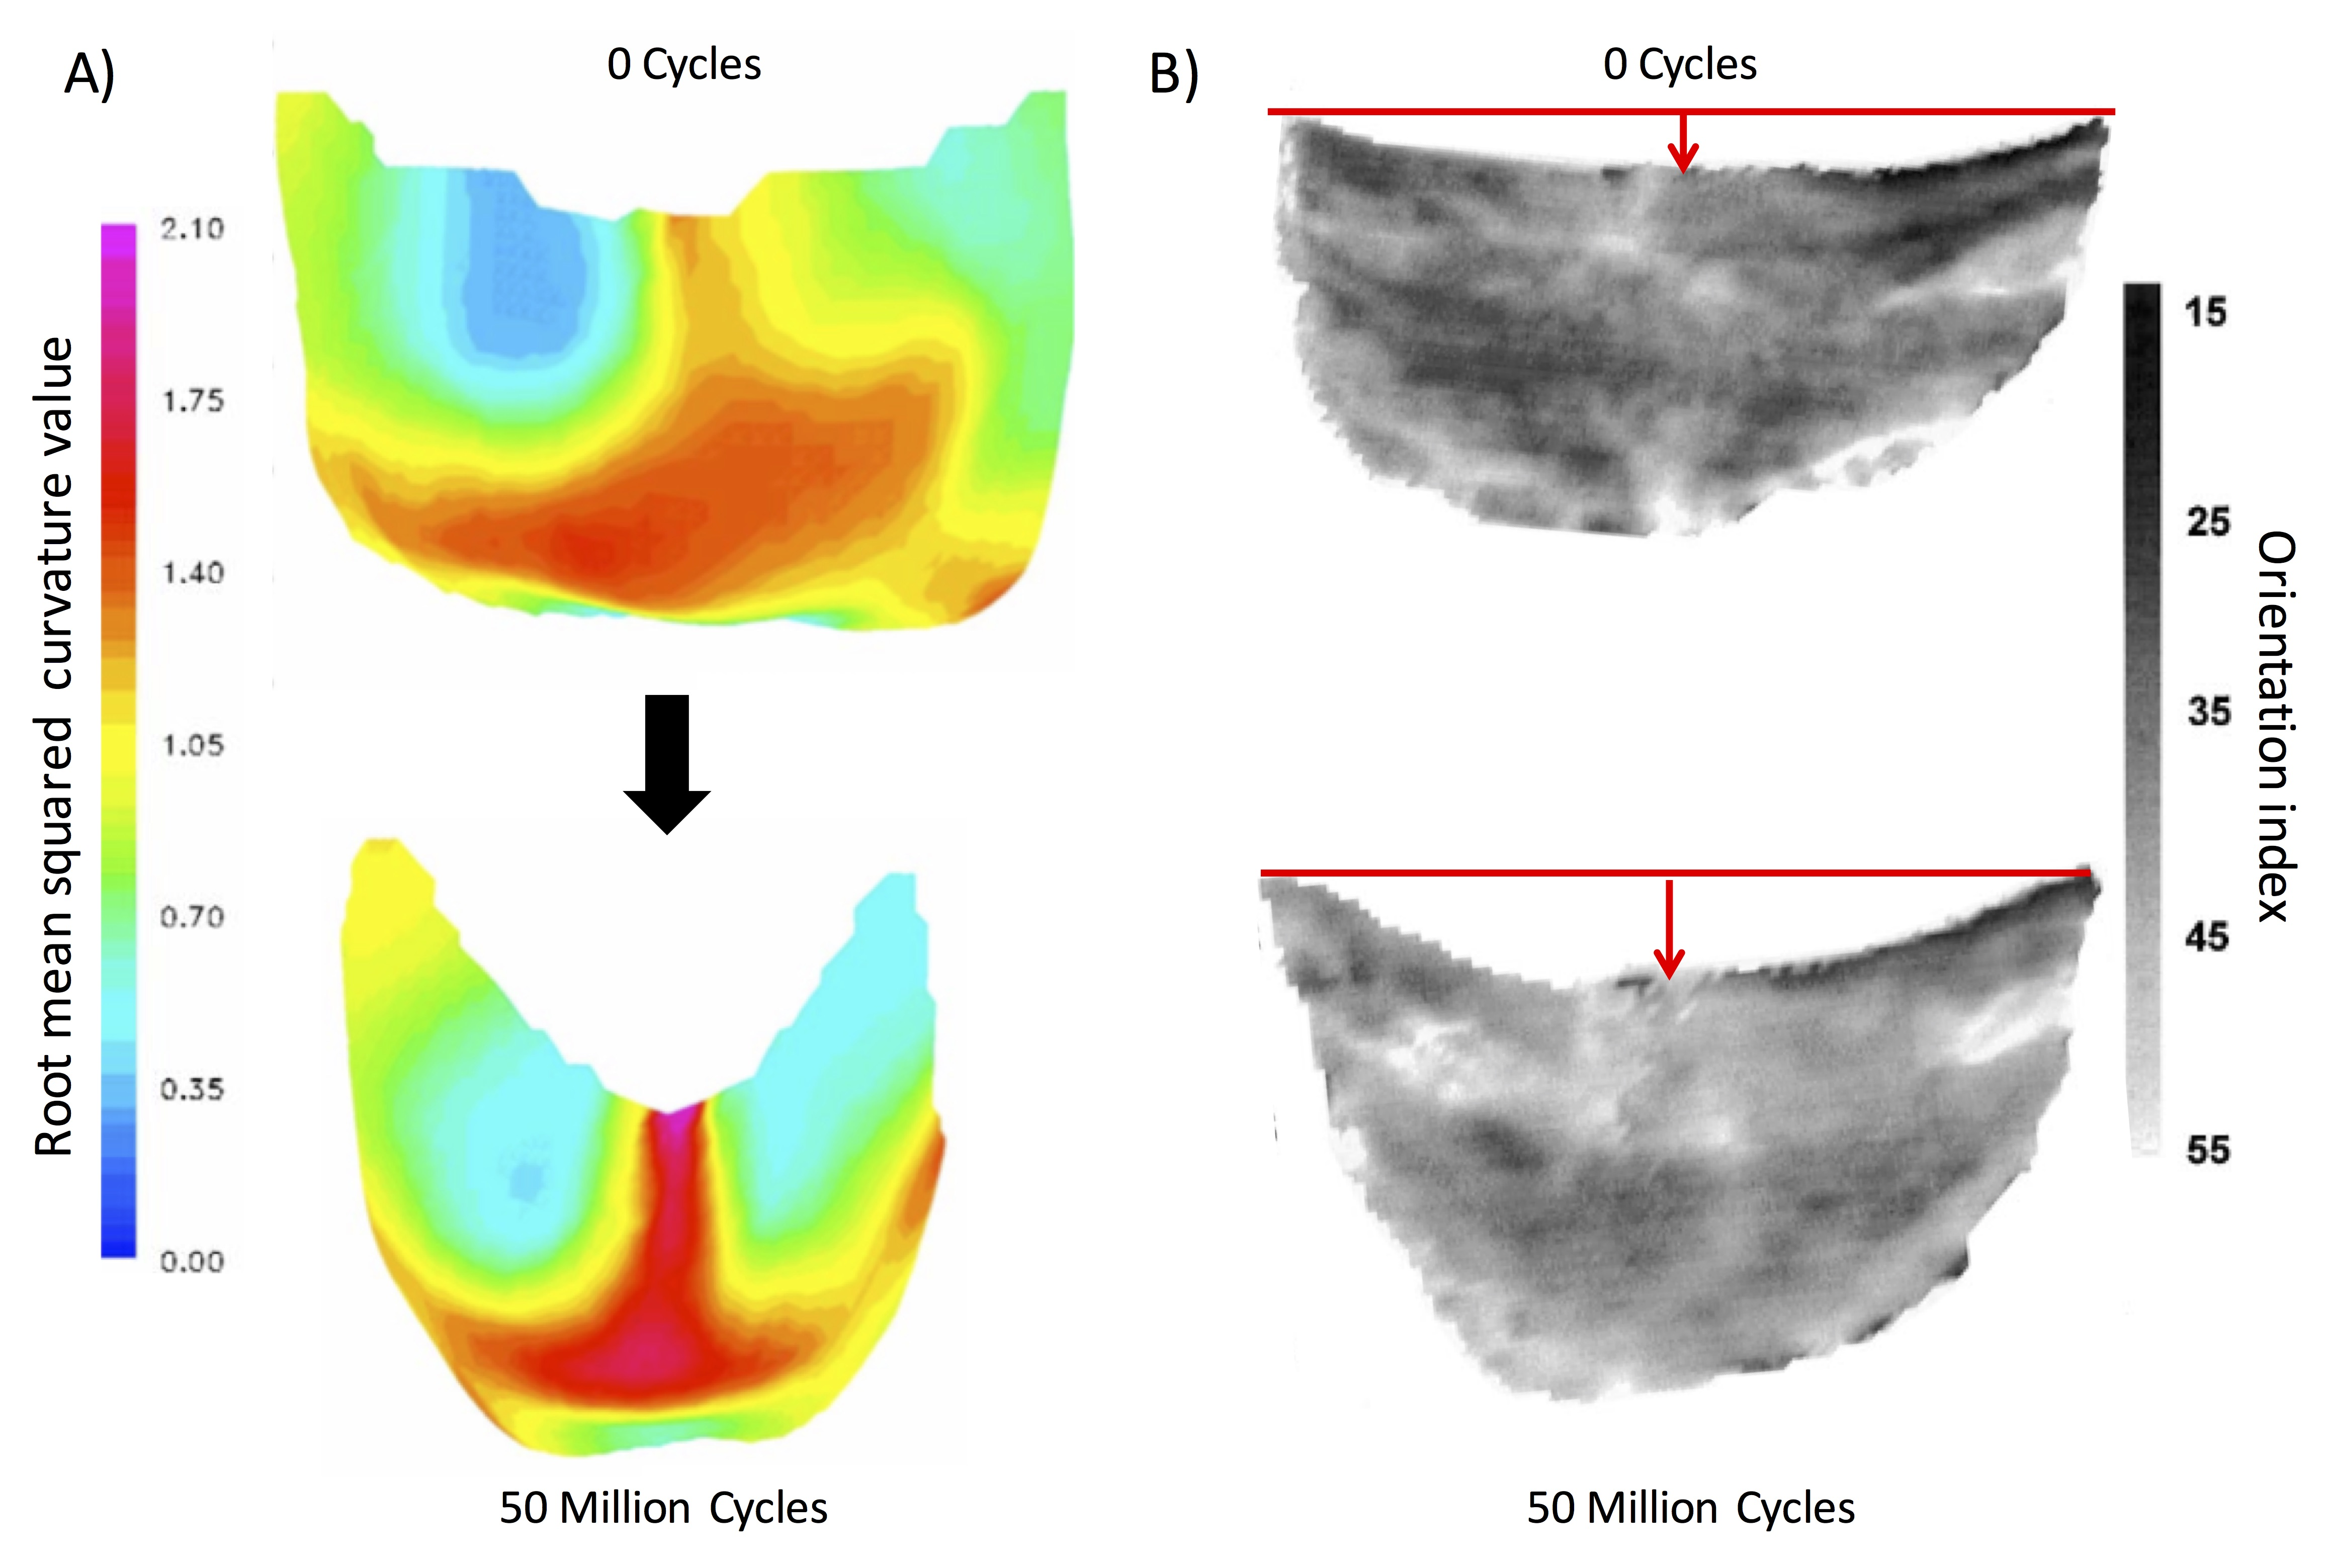
\includegraphics[width=\textwidth]{Images/chapter4/figure1}
\caption{A) The 3D unloaded geometry a BHV leaflet before and after cyclic loading, with the color indicating the local root mean squared curvature. The most significant change in geometry is in the belly region. B) BHV leaflet collagen fiber architecture, showing that the collagen fiber architecture are convected by the dimensional changes. The grayscale scale bar shows the orientation index (OI), which is angle containing 50 \% of fibers. The lack of changes in the OI suggests that minimal damage to the collagen fiber architecture has occurred.}
\label{fig:PSeffects}
\end{figure}


%%%%%%%%%%%%%%%%%%%%%%%%%%%%%%%%%%%%%%%%%%%%%%%%%%%%%%%%%%%%%%%%%%%%%%%%%%%%%%%%
%%%%    Exogenous crosslinking

\subsection{The effect of exogenous crosslinking}

	Bovine pericardium (BP) is a dense collagenous tissue composed mostly of collagen type I fibers with some elastin, GAGs, cells and vasculature. Collagen fibers are complex protein structures at the 2 - 10 $\mu$m scale, composed of tightly bundled collagen fibrils, which are approximately 50 nm in diameter. Much of what we know about the use of GLUT to exogenously crosslink collagenous tissue is from Nimni \textit{et al.} \cite{cheung_mechanism_1990, nimni_chemically_1987, cheung_mechanism_1985, gendler_toxic_1984, cheung_presence_1983, cheung_mechanism_1982, cheung_mechanism_1982II}. GLUT, which is an aldehyde based crosslinker, aggressively crosslinks free amines in proteins. This suppresses immunogenicity by crosslinking all cell membrane protein remnants, but also forms polymeric networks (at the nm scale) which allow for long range crosslinks to the nearby tissue microstructures. We previously found that exogenous crosslinking increases the bending stiffness of the matrix by four time the original stiffness \cite{mirnajafi_effects_2010}. We also tested the mechanical response of exogenously crosslinked BP before and after crosslinking, and developed the first constitutive model for exogenously crosslinked soft tissue \cite{sacks_novel_2016}. Interestingly, we also found that exogenously crosslinking does not increase the collagen fiber modulus, but significantly increases the interactions between collagen fibers \cite{sacks_novel_2016}, which is responsible for up to 30\% of the stress in the fully loaded state. 


	The GLUT crosslinking process involves a Schiff-base reaction. Importantly, the molecular bonds formed from Schiff-base reactions are known to be unstable at room and temperatures \cite{migneault_glutaraldehyde_2004, damink_glutaraldehyde_1995}. Thus, although GLUT is highly reactive and aggressively crosslinks extracellular matrix proteins, any resulting crosslinks will also readily undergo hydrolysis at body temperature \cite{migneault_glutaraldehyde_2004}. As a result, under cyclic loading in-vivo, exogenous ECM crosslinks will constantly break and reform. This continual process will cause the reference configuration to evolve towards the current loaded state. \emph{We thus hypothesize that this scission-healing behavior could be linked to the mechanisms that underlie how the BHV leaflet geometry evolves over time}.
	
	
    This damageless change in the BHV geometry has many similarities to the permanent set (PS) mechanisms observed in elastomers. Permanent set is an irreversible deformation that remains after a structure or material has been subjected to external stresses and then released. It does not involve damage to the constituents of the material, but instead changes the referential configuration. Although the outcomes may be similar, \emph{this form of permanent set is not a plastic deformations}, as they are entirely within the elastic regime. In particular, it has been used to model the scission-healing reactions of elastomers that occur when stretched, heated, cooled, then unloaded. This results in some of the materials to change in referential configuration to the loaded state. In this process, permanent set does not damage the polymeric fibers but is a result of the change in configuration of the underlying polymeric fiber network. Some works on constitutive models of this process include the works of Rajagopal and Wineman \cite{rajagopal_constitutive_1992}, Andrews and Tobolsky \cite{andrews_theory_1946}, and Rottach \textit{et al}. \cite{rottach_effect_2004, rottach_molecular_2007, rottach_permanent_2006}. However, there are little known studies on the permanent set effect in soft tissues or soft tissue derived exogenously crosslinked biomaterials. 
	

	\emph{Based on the above considerations, we hypothesize that the initial time evolving BHV geometry and mechanical response can be predicted by permanent set mechanisms}. Rather than heating and cooling, we assume that permanent set in exogenously crosslinked tissue occurs continuously at body temperature due to the GLUT, allowing the reference configuration of the exogenously crosslinked matrix (EXL matrix) to evolve over time. As a result, the reference configuration of BHVs will change while not affecting the intrinsic material properties of their constituents such as collagen fibers and the EXL matrix. Since the BHVs deform into a new configuration (Fig. \ref{fig:PSeffects}), there may develop regions of stress concentrations. The high stresses will increase the rate of structural damage and thus accelerate the rate of BHV failure. Thus, \emph{by compensating for the permanent set effects, it may be possible to reduce the BHV leaflet stresses and thus reduce structural damage to BHVs during \textit{in vivo} operation after implant.} Therefore, constitutive models that can predict the effects of permanent set are crucial for the simulation of BHVs. 

		
%%%%%%%%%%%%%%%%%%%%%%%%%%%%%%%%%%%%%%%%%%%%%%%%%%%%%%%%%%%%%%%%%%%%%%%%%%%%%%%%
%%%%    Constitutive models

\subsection{Constitutive models for the permanent set effect for soft tissues}

	The only work in the simulation of the permanent set effect in native or exogenously crosslinked soft tissues is the pioneering study of Martin and Sun \cite{martin_modeling_2013}, who developed a time dependent constitutive model for uniaxial cyclic loading of GLUT exogenously crosslinked BP strips using a damage analog. Briefly, to model the uncycled mechanical response, they used the Fung hyperelastic model for the strain energy density function, $\Psi_0$. The time dependent stress softening was then described using a modification to the strain energy function as $\Psi_\mathrm{PS} = (1-D_s)\Psi_0 - \Psi_0(\mathbf{E}_\mathrm{PS})$. Here the strain energy of the material after permanent set ($\Psi_\mathrm{PS}$) is reduced from $\Psi_0$ in accordance with a scaled damage function $D_s$ and the same strain energy function evaluated at the current amount of permanent set ($\mathbf{E}_\mathrm{PS}$). Martin and Sun then measured the maximum permanent set deformation that occurs for each specimen, and used that to set the maximum bound of $\mathbf{E}_\mathrm{PS}$. Additionally, Martin and Sun set two parameters, a lowerbound below which no permanent set occurs, and an upperbound above which the tissue fails. In the intermediate region, $D_s$ and $\mathbf{E}_\mathrm{PS}$ simply increase linearly with the number of cycles. The number of cycles needed to reach the maximum permanent set deformation was then described using an inverse exponential like function of the maximum strain applied, which is an analogous to the stress versus cycles (S–N) curve used to describe the fatigue behavior of traditional engineering materials. However, such approaches have the following limitations: 1) they are not predictive as there are no underlying mechanisms in the model. A damage-like model can mimic the results of permanent set but cannot explain nor predict the mechanisms responsible in exogenously crosslinked tissue, and 2) there is no way to extrapolate for predicting into unmeasured regimes using the Fung hyperelastic model. Therefore, there is a need for a more predictive constitutive model that utilizes the underlying mechanisms.


%%%%%%%%%%%%%%%%%%%%%%%%%%%%%%%%%%%%%%%%%%%%%%%%%%%%%%%%%%%%%%%%%%%%%%%%%%%%%%%%
%%%%    A new approach

\subsection{A new approach for modeling the permanent set effect in exogenously crosslinked soft tissues}

	We utilize a structural constitutive modeling approach, which integrates information on tissue composition and structure for material characterization \cite{sacks_structural_2000}. In principal, using structural models we only need to perform parameter estimation for the intrinsic material properties, such as collagen fiber modulus and EXL matrix modulus, to predict the mechanical response using the quantified tissue microstructure. This mechanism based approach allows us to predict the mechanical response at strains outside of the strain range of the experimental data used for parameter estimation \cite{zhang_meso_2016, fata_insights_2014}; a feat not possible using purely phenomenological approaches. In addition, by using a structural modeling approach coupled with the permanent set mechanism to predict the collagen fiber architecture after cyclic loading, we can also predict the mechanical response of the soft tissue at higher cycle numbers. Thus, we use 1) the structural model parameters obtained in the uncycled mechanical state and 2) the permanent set mechanisms to predict how the mechanical response of the exogenously crosslinked tissues evolves with cyclic loading. The key aspects of our approach include:
\begin{enumerate}
\item Model the change in mechanical response entirely as a kinematic change in the underlying microstructure; no actual change in mechanical properties (damage)
\item Predict the change in geometry from the loading history and the permanent set mechanism
\item Validate the permanent set mechanism under both strain and stress controlled loading conditions
\item Develop a time dependent implementation with an evolving loaded configuration under stress control
\end{enumerate}